\documentclass[tikz]{standalone}

% \usepackage{newtxtext,newtxmath}

% mytikzset
\usepackage{tikz}
\usetikzlibrary{positioning,arrows,shapes}
\usetikzlibrary{decorations.pathmorphing}
\usetikzlibrary{decorations.markings}
\usetikzlibrary{shapes.arrows, fadings}
\usetikzlibrary{shapes,snakes}
\usetikzlibrary{calc}

\tikzset{
  vector/.style={thick,double,draw=black, postaction={decorate},
    decoration={markings,mark=at position .6 with {\arrow[black,scale=0.4]{triangle 45}}}},
  axial/.style={thick,double,densely dashed,draw=black, postaction={decorate},
    decoration={markings,mark=at position .6 with {\arrow[black,scale=0.4]{triangle 45}}}},
  gluon/.style={decorate, draw=black,
    decoration={coil,aspect=0.3,segment length=5pt,amplitude=3pt}},
  pseudo/.style={thick, dashed, draw=black, postaction={decorate},
    decoration={markings,mark=at position .6 with {\arrow[red,scale=0.5]{triangle 45}}}},
  scalar/.style={thick,draw=black, postaction={decorate},
    decoration={markings,mark=at position .6 with {\arrow[black,scale=0.5]{triangle 45}}}}%,
  % pomeron/.style={thick,draw=black, postaction={decorate},
  % decoration={zigzag,segment length=4,amplitude=.9}}
}

\definecolor{myGreen}{RGB}{0,127,0}

\begin{document}
\nopagecolor
  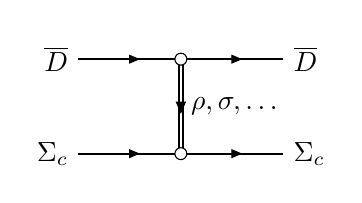
\begin{tikzpicture}[x=1.3cm, y=0.6cm, baseline=1cm]
    \node[coordinate] (A) at ( 0, 1) {};
    \node[coordinate] (B) at ( 0,-1) {};
    \draw[scalar] (-1, 1) node[left] {$\overline{D}$} -- (A);
    \draw[scalar] (-1,-1) node[left] {$\Sigma_c$} -- (B);
    \draw[scalar] (A) -- ( 1,1) node[right] {$\overline{D}$};
    \draw[scalar] (B) -- ( 1,-1) node[right] {$\Sigma_c$};
    %
    \draw[vector] (A) -- node[right] {$\rho,\sigma,\dots$} (B);
    \draw[black, fill=white] (A) circle (0.5ex);
    \draw[black, fill=white] (B) circle (0.5ex);
    % \draw [decorate,decoration={brace,amplitude=3pt}] ($(A)+(0.2,0.1)$) -- ($(B)+(0.2,-0.1)$) node [black,midway,xshift=0.3cm] {$s$};
  \end{tikzpicture}
\end{document}
